% -*- Mode:TeX -*-

%% IMPORTANT: The official thesis specifications are available at:
%%            http://libraries.mit.edu/archives/thesis-specs/
%%
%%            Please verify your thesis' formatting and copyright
%%            assignment before submission.  If you notice any
%%            discrepancies between these templates and the 
%%            MIT Libraries' specs, please let us know
%%            by e-mailing thesis@mit.edu

%% The documentclass options along with the pagestyle can be used to generate
%% a technical report, a draft copy, or a regular thesis.  You may need to
%% re-specify the pagestyle after you \include  cover.tex.  For more
%% information, see the first few lines of mitthesis.cls. 

%\documentclass[12pt,vi,twoside]{mitthesis}
%%
%%  If you want your thesis copyright to you instead of MIT, use the
%%  ``vi'' option, as above.
%%
%\documentclass[12pt,twoside,leftblank]{mitthesis}
%%
%% If you want blank pages before new chapters to be labelled ``This
%% Page Intentionally Left Blank'', use the ``leftblank'' option, as
%% above. 

\documentclass[12pt,twoside]{mitthesis}
\usepackage{lgrind}
%% These have been added at the request of the MIT Libraries, because
%% some PDF conversions mess up the ligatures.  -LB, 1/22/2014
\usepackage{cmap}
\usepackage[T1]{fontenc}
\pagestyle{plain}
\usepackage{graphicx}
\usepackage{hyperref}

%% This bit allows you to either specify only the files which you wish to
%% process, or `all' to process all files which you \include.
%% Krishna Sethuraman (1990).

%\typein [\files]{Enter file names to process, (chap1,chap2 ...), or `all' to
%process all files:}
\def\all{all}
%\ifx\files\all \typeout{Including all files.} \else \typeout{Including only \files.} \includeonly{\files} \fi

\begin{document}

% -*-latex-*-
% 
% For questions, comments, concerns or complaints:
% thesis@mit.edu
% 
%
% $Log: cover.tex,v $
% Revision 1.8  2008/05/13 15:02:15  jdreed
% Degree month is June, not May.  Added note about prevdegrees.
% Arthur Smith's title updated
%
% Revision 1.7  2001/02/08 18:53:16  boojum
% changed some \newpages to \cleardoublepages
%
% Revision 1.6  1999/10/21 14:49:31  boojum
% changed comment referring to documentstyle
%
% Revision 1.5  1999/10/21 14:39:04  boojum
% *** empty log message ***
%
% Revision 1.4  1997/04/18  17:54:10  othomas
% added page numbers on abstract and cover, and made 1 abstract
% page the default rather than 2.  (anne hunter tells me this
% is the new institute standard.)
%
% Revision 1.4  1997/04/18  17:54:10  othomas
% added page numbers on abstract and cover, and made 1 abstract
% page the default rather than 2.  (anne hunter tells me this
% is the new institute standard.)
%
% Revision 1.3  93/05/17  17:06:29  starflt
% Added acknowledgements section (suggested by tompalka)
% 
% Revision 1.2  92/04/22  13:13:13  epeisach
% Fixes for 1991 course 6 requirements
% Phrase "and to grant others the right to do so" has been added to 
% permission clause
% Second copy of abstract is not counted as separate pages so numbering works
% out
% 
% Revision 1.1  92/04/22  13:08:20  epeisach

% NOTE:
% These templates make an effort to conform to the MIT Thesis specifications,
% however the specifications can change.  We recommend that you verify the
% layout of your title page with your thesis advisor and/or the MIT 
% Libraries before printing your final copy.
\title{An approach to a Disaster Preparedness System}

\author{Mohammed Faisal Khan}
% If you wish to list your previous degrees on the cover page, use the 
% previous degrees command:
%       \prevdegrees{A.A., Harvard University (1985)}
% You can use the \\ command to list multiple previous degrees
%       \prevdegrees{B.S., University of California (1978) \\
%                    S.M., Massachusetts Institute of Technology (1981)}
\department{Department of Computer Science}

% If the thesis is for two degrees simultaneously, list them both
% separated by \and like this:
% \degree{Doctor of Philosophy \and Master of Science}
\degree{Master of Science in Computer Science}

% As of the 2007-08 academic year, valid degree months are September, 
% February, or June.  The default is June.
\degreemonth{December}
\degreeyear{2018}
\thesisdate{May 1, 2018}

%% By default, the thesis will be copyrighted to MIT.  If you need to copyright
%% the thesis to yourself, just specify the `vi' documentclass option.  If for
%% some reason you want to exactly specify the copyright notice text, you can
%% use the \copyrightnoticetext command.  
%\copyrightnoticetext{\copyright IBM, 1990.  Do not open till Xmas.}
\copyrightnoticetext{\copyright University of New Haven, 2018}

% If there is more than one supervisor, use the \supervisor command
% once for each.
\supervisor{Amir Esmailpour}{Associate Professor}

% This is the department committee chairman, not the thesis committee
% chairman.  You should replace this with your Department's Committee
% Chairman.
\chairman{Ronald S. Harichandran}{Chairman, Department Committee on Graduate Theses}

% Make the titlepage based on the above information.  If you need
% something special and can't use the standard form, you can specify
% the exact text of the titlepage yourself.  Put it in a titlepage
% environment and leave blank lines where you want vertical space.
% The spaces will be adjusted to fill the entire page.  The dotted
% lines for the signatures are made with the \signature command.
\maketitle

% The abstractpage environment sets up everything on the page except
% the text itself.  The title and other header material are put at the
% top of the page, and the supervisors are listed at the bottom.  A
% new page is begun both before and after.  Of course, an abstract may
% be more than one page itself.  If you need more control over the
% format of the page, you can use the abstract environment, which puts
% the word "Abstract" at the beginning and single spaces its text.

%% You can either \input (*not* \include) your abstract file, or you can put
%% the text of the abstract directly between the \begin{abstractpage} and
%% \end{abstractpage} commands.

% First copy: start a new page, and save the page number.
\cleardoublepage
% Uncomment the next line if you do NOT want a page number on your
% abstract and acknowledgments pages.
% \pagestyle{empty}
\setcounter{savepage}{\thepage}
\begin{abstractpage}
% $Log: abstract.tex,v $
% Revision 1.1  93/05/14  14:56:25  starflt
% Initial revision
% 
% Revision 1.1  90/05/04  10:41:01  lwvanels
% Initial revision
% 
%
%% The text of your abstract and nothing else (other than comments) goes here.
%% It will be single-spaced and the rest of the text that is supposed to go on
%% the abstract page will be generated by the abstractpage environment.  This
%% file should be \input (not \include 'd) from cover.tex.
In this thesis, I designed and implemented a disaster management platform which collects data from social media platform like twitter in real time using stream listener and stores the information in MongoDB, a NoSQL database, which is used to parsed the tweets. Hadoop map and reduce was used to extract related and meaningful data from the tweets which can be used directly using the provided API as well as have various applications using Machine Learning algorithms for modelling the various disaster scenarios. The data extracted was used to provide information about the resources available during a disaster like shelter capacity, food provisions and safe zones.
\end{abstractpage}

% Additional copy: start a new page, and reset the page number.  This way,
% the second copy of the abstract is not counted as separate pages.
% Uncomment the next 6 lines if you need two copies of the abstract
% page.
% \setcounter{page}{\thesavepage}
% \begin{abstractpage}
% % $Log: abstract.tex,v $
% Revision 1.1  93/05/14  14:56:25  starflt
% Initial revision
% 
% Revision 1.1  90/05/04  10:41:01  lwvanels
% Initial revision
% 
%
%% The text of your abstract and nothing else (other than comments) goes here.
%% It will be single-spaced and the rest of the text that is supposed to go on
%% the abstract page will be generated by the abstractpage environment.  This
%% file should be \input (not \include 'd) from cover.tex.
In this thesis, I designed and implemented a disaster management platform which collects data from social media platform like twitter in real time using stream listener and stores the information in MongoDB, a NoSQL database, which is used to parsed the tweets. Hadoop map and reduce was used to extract related and meaningful data from the tweets which can be used directly using the provided API as well as have various applications using Machine Learning algorithms for modelling the various disaster scenarios. The data extracted was used to provide information about the resources available during a disaster like shelter capacity, food provisions and safe zones.
% \end{abstractpage}

\cleardoublepage

\section*{Acknowledgments}

This is the acknowledgements section.  You should replace this with your
own acknowledgements.

%%%%%%%%%%%%%%%%%%%%%%%%%%%%%%%%%%%%%%%%%%%%%%%%%%%%%%%%%%%%%%%%%%%%%%
% -*-latex-*-

% Some departments (e.g. 5) require an additional signature page.  See
% signature.tex for more information and uncomment the following line if
% applicable.
% % -*- Mode:TeX -*-
%
% Some departments (e.g. Chemistry) require an additional cover page
% with signatures of the thesis committee.  Please check with your
% thesis advisor or other appropriate person to determine if such a 
% page is required for your thesis.  
%
% If you choose not to use the "titlepage" environment, a \newpage
% commands, and several \vspace{\fill} commands may be necessary to
% achieve the required spacing.  The \signature command is defined in
% the "mitthesis" class
%
% The following sample appears courtesy of Ben Kaduk <kaduk@mit.edu> and
% was used in his June 2012 doctoral thesis in Chemistry. 

\begin{titlepage}
\begin{large}
This doctoral thesis has been examined by a Committee of the Department
of Chemistry as follows:

\signature{Professor Jianshu Cao}{Chairman, Thesis Committee \\
   Professor of Chemistry}

\signature{Professor Troy Van Voorhis}{Thesis Supervisor \\
   Associate Professor of Chemistry}

\signature{Professor Robert W. Field}{Member, Thesis Committee \\
   Haslam and Dewey Professor of Chemistry}
\end{large}
\end{titlepage}


\pagestyle{plain}
  % -*- Mode:TeX -*-
%% This file simply contains the commands that actually generate the table of
%% contents and lists of figures and tables.  You can omit any or all of
%% these files by simply taking out the appropriate command.  For more
%% information on these files, see appendix C.3.3 of the LaTeX manual. 
\tableofcontents
\newpage
\listoffigures
\newpage
\listoftables


%% This is an example first chapter.  You should put chapter/appendix that you
%% write into a separate file, and add a line \include{yourfilename} to
%% main.tex, where `yourfilename.tex' is the name of the chapter/appendix file.
%% You can process specific files by typing their names in at the 
%% \files=
%% prompt when you run the file main.tex through LaTeX.
\chapter{Introduction}

Micro-optimization is a technique to reduce the overall operation count of
floating point operations.  In a standard floating point unit, floating
point operations are fairly high level, such as ``multiply'' and ``add'';
in a micro floating point unit ($\mu$FPU), these have been broken down into
their constituent low-level floating point operations on the mantissas and
exponents of the floating point numbers.

Chapter two describes the architecture of the $\mu$FPU unit, and the
motivations for the design decisions made.

Chapter three describes the design of the compiler, as well as how the
optimizations discussed in section~\ref{ch1:opts} were implemented.

Chapter four describes the purpose of test code that was compiled, and which
statistics were gathered by running it through the simulator.  The purpose
is to measure what effect the micro-optimizations had, compared to
unoptimized code.  Possible future expansions to the project are also
discussed.

\section{Motivations for micro-optimization}

The idea of micro-optimization is motivated by the recent trends in computer
architecture towards low-level parallelism and small, pipelineable
instruction sets \cite{patterson:risc,rad83}.  By getting rid of more
complex instructions and concentrating on optimizing frequently used
instructions, substantial increases in performance were realized.

Another important motivation was the trend towards placing more of the
burden of performance on the compiler.  Many of the new architectures depend
on an intelligent, optimizing compiler in order to realize anywhere near
their peak performance
\cite{ellis:bulldog,pet87,coutant:precision-compilers}.  In these cases, the
compiler not only is responsible for faithfully generating native code to
match the source language, but also must be aware of instruction latencies,
delayed branches, pipeline stages, and a multitude of other factors in order
to generate fast code \cite{gib86}.

Taking these ideas one step further, it seems that the floating point
operations that are normally single, large instructions can be further broken
down into smaller, simpler, faster instructions, with more control in the
compiler and less in the hardware.  This is the idea behind a
micro-optimizing FPU; break the floating point instructions down into their
basic components and use a small, fast implementation, with a large part of
the burden of hardware allocation and optimization shifted towards
compile-time.

Along with the hardware speedups possible by using a $\mu$FPU, there are
also optimizations that the compiler can perform on the code that is
generated.  In a normal sequence of floating point operations, there are
many hidden redundancies that can be eliminated by allowing the compiler to
control the floating point operations down to their lowest level.  These
optimizations are described in detail in section~\ref{ch1:opts}.

\section{Description of micro-optimization}\label{ch1:opts}

In order to perform a sequence of floating point operations, a normal FPU
performs many redundant internal shifts and normalizations in the process of
performing a sequence of operations.  However, if a compiler can
decompose the floating point operations it needs down to the lowest level,
it then can optimize away many of these redundant operations.  

If there is some additional hardware support specifically for
micro-optimization, there are additional optimizations that can be
performed.  This hardware support entails extra ``guard bits'' on the
standard floating point formats, to allow several unnormalized operations to
be performed in a row without the loss information\footnote{A description of
the floating point format used is shown in figures~\ref{exponent-format}
and~\ref{mantissa-format}.}.  A discussion of the mathematics behind
unnormalized arithmetic is in appendix~\ref{unnorm-math}.

The optimizations that the compiler can perform fall into several categories:

\subsection{Post Multiply Normalization}

When more than two multiplications are performed in a row, the intermediate
normalization of the results between multiplications can be eliminated.
This is because with each multiplication, the mantissa can become
denormalized by at most one bit.  If there are guard bits on the mantissas
to prevent bits from ``falling off'' the end during multiplications, the
normalization can be postponed until after a sequence of several
multiplies\footnote{Using unnormalized numbers for math is not a new idea; a
good example of it is the Control Data CDC 6600, designed by Seymour Cray.
\cite{thornton:cdc6600} The CDC 6600 had all of its instructions performing
unnormalized arithmetic, with a separate {\tt NORMALIZE} instruction.}.

% This is an example of how you would use tgrind to include an example
% of source code; it is commented out in this template since the code
% example file does not exist.  To use it, you need to remove the '%' on the
% beginning of the line, and insert your own information in the call.
%
%\tagrind[htbp]{code/pmn.s.tex}{Post Multiply Normalization}{opt:pmn}

As you can see, the intermediate results can be multiplied together, with no
need for intermediate normalizations due to the guard bit.  It is only at
the end of the operation that the normalization must be performed, in order
to get it into a format suitable for storing in memory\footnote{Note that
for purposed of clarity, the pipeline delays were considered to be 0, and
the branches were not delayed.}.

\subsection{Block Exponent}

In a unoptimized sequence of additions, the sequence of operations is as
follows for each pair of numbers ($m_1$,$e_1$) and ($m_2$,$e_2$).
\begin{enumerate}
  \item Compare $e_1$ and $e_2$.
  \item Shift the mantissa associated with the smaller exponent $|e_1-e_2|$
        places to the right.
  \item Add $m_1$ and $m_2$.
  \item Find the first one in the resulting mantissa.
  \item Shift the resulting mantissa so that normalized
  \item Adjust the exponent accordingly.
\end{enumerate}

Out of 6 steps, only one is the actual addition, and the rest are involved
in aligning the mantissas prior to the add, and then normalizing the result
afterward.  In the block exponent optimization, the largest mantissa is
found to start with, and all the mantissa's shifted before any additions
take place.  Once the mantissas have been shifted, the additions can take
place one after another\footnote{This requires that for n consecutive
additions, there are $\log_{2}n$ high guard bits to prevent overflow.  In
the $\mu$FPU, there are 3 guard bits, making up to 8 consecutive additions
possible.}.  An example of the Block Exponent optimization on the expression
X = A + B + C is given in figure~\ref{opt:be}.

% This is an example of how you would use tgrind to include an example
% of source code; it is commented out in this template since the code
% example file does not exist.  To use it, you need to remove the '%' on the
% beginning of the line, and insert your own information in the call.
%
%\tgrind[htbp]{code/be.s.tex}{Block Exponent}{opt:be}

\section{Integer optimizations}

As well as the floating point optimizations described above, there are
also integer optimizations that can be used in the $\mu$FPU.  In concert
with the floating point optimizations, these can provide a significant
speedup.  

\subsection{Conversion to fixed point}

Integer operations are much faster than floating point operations; if it is
possible to replace floating point operations with fixed point operations,
this would provide a significant increase in speed.

This conversion can either take place automatically or or based on a
specific request from the programmer.  To do this automatically, the
compiler must either be very smart, or play fast and loose with the accuracy
and precision of the programmer's variables.  To be ``smart'', the computer
must track the ranges of all the floating point variables through the
program, and then see if there are any potential candidates for conversion
to floating point.  This technique is discussed further in
section~\ref{range-tracking}, where it was implemented.

The other way to do this is to rely on specific hints from the programmer
that a certain value will only assume a specific range, and that only a
specific precision is desired.  This is somewhat more taxing on the
programmer, in that he has to know the ranges that his values will take at
declaration time (something normally abstracted away), but it does provide
the opportunity for fine-tuning already working code.

Potential applications of this would be simulation programs, where the
variable represents some physical quantity; the constraints of the physical
system may provide bounds on the range the variable can take.
\subsection{Small Constant Multiplications}

One other class of optimizations that can be done is to replace
multiplications by small integer constants into some combination of
additions and shifts.  Addition and shifting can be significantly faster
than multiplication.  This is done by using some combination of
\begin{eqnarray*}
a_i & = & a_j + a_k \\
a_i & = & 2a_j + a_k \\
a_i & = & 4a_j + a_k \\
a_i & = & 8a_j + a_k \\
a_i & = & a_j - a_k \\
a_i & = & a_j \ll m \mbox{shift}
\end{eqnarray*}
instead of the multiplication.  For example, to multiply $s$ by 10 and store
the result in $r$, you could use:
\begin{eqnarray*}
r & = & 4s + s\\
r & = & r + r
\end{eqnarray*}
Or by 59:
\begin{eqnarray*}
t & = & 2s + s \\
r & = & 2t + s \\
r & = & 8r + t
\end{eqnarray*}
Similar combinations can be found for almost all of the smaller
integers\footnote{This optimization is only an ``optimization'', of course,
when the amount of time spent on the shifts and adds is less than the time
that would be spent doing the multiplication.  Since the time costs of these
operations are known to the compiler in order for it to do scheduling, it is
easy for the compiler to determine when this optimization is worth using.}.
\cite{magenheimer:precision}

\section{Other optimizations}

\subsection{Low-level parallelism}

The current trend is towards duplicating hardware at the lowest level to
provide parallelism\footnote{This can been seen in the i860; floating point
additions and multiplications can proceed at the same time, and the RISC
core be moving data in and out of the floating point registers and providing
flow control at the same time the floating point units are active. \cite{byte:i860}}

Conceptually, it is easy to take advantage to low-level parallelism in the
instruction stream by simply adding more functional units to the $\mu$FPU,
widening the instruction word to control them, and then scheduling as many
operations to take place at one time as possible.

However, simply adding more functional units can only be done so many times;
there is only a limited amount of parallelism directly available in the
instruction stream, and without it, much of the extra resources will go to
waste.  One process used to make more instructions potentially schedulable
at any given time is ``trace scheduling''.  This technique originated in the
Bulldog compiler for the original VLIW machine, the ELI-512.
\cite{ellis:bulldog,colwell:vliw}  In trace scheduling, code can be
scheduled through many basic blocks at one time, following a single
potential ``trace'' of program execution.  In this way, instructions that
{\em might\/} be executed depending on a conditional branch further down in
the instruction stream are scheduled, allowing an increase in the potential
parallelism.  To account for the cases where the expected branch wasn't
taken, correction code is inserted after the branches to undo the effects of
any prematurely executed instructions.

\subsection{Pipeline optimizations}

In addition to having operations going on in parallel across functional
units, it is also typical to have several operations in various stages of
completion in each unit.  This pipelining allows the throughput of the
functional units to be increased, with no increase in latency.

There are several ways pipelined operations can be optimized.  On the
hardware side, support can be added to allow data to be recirculated back
into the beginning of the pipeline from the end, saving a trip through the
registers.  On the software side, the compiler can utilize several tricks to
try to fill up as many of the pipeline delay slots as possible, as
seendescribed by Gibbons. \cite{gib86}



%% This is an example first chapter.  You should put chapter/appendix that you
%% write into a separate file, and add a line \include{yourfilename} to
%% main.tex, where `yourfilename.tex' is the name of the chapter/appendix file.
%% You can process specific files by typing their names in at the 
%% \files=
%% prompt when you run the file main.tex through LaTeX.
\chapter{Design}

\begin{figure}[ht!]
	\centering
	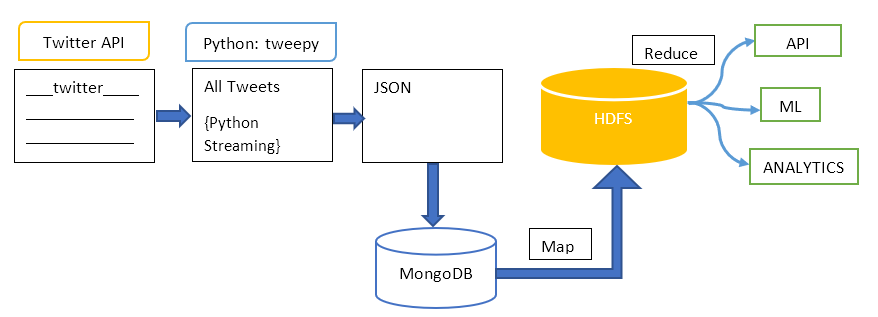
\includegraphics[width=150mm]{DesignDiagram.png}
	\caption{A simple caption \label{overflow}}
\end{figure}

\section{Twitter}

\subsection{Twitter API}\label{ch1:opts}

Twitter as a platform has a lot of users and it generates a lot of data that can be used for analysis. Data can include user tweets, user profiles, user friends and followers, what’s trending, etc. This data can be extracted using twitter Application Programming Interface(API). There are three methods to get this data: the REST API, the search API, and the Streaming API. The Search API is retrospective and allows you search old tweets [with severe limitations], the REST API allows you to collect user profiles, friends, and followers, and the Streaming API collects tweets in real time as they happen. As we are going to do a real time analysis of the data we find the Streaming API most suited to our needs.

The Twitter API requires a few steps:

\begin{enumerate}
  \item Authenticate with OAuth
  \item Make API call
  \item Receive JSON file back
  \item Interpret JSON file
\end{enumerate}

\subsection{Authenticate with OAuth}

OAuth is an open standard for access delegation, commonly used as a way for internet users to grant websites or applications access to their information on other websites or applications access to their information on other websites but without giving them the passwords (Gordon, 2012). Authentication with OAuth on Twitter requires you to get keys from the Twitter developers site using a Twitter developer account. There are four keys (Consumer Key, Consumer Secret Key, Access Token, and Secret Token) that are required to access the API and need to be used during a handshake, once authenticated the program can make API calls.

% This is an example of how you would use tgrind to include an example
% of source code; it is commented out in this template since the code
% example file does not exist.  To use it, you need to remove the '%' on the
% beginning of the line, and insert your own information in the call.
%
%\tagrind[htbp]{code/pmn.s.tex}{Post Multiply Normalization}{opt:pmn}

\subsection{Make API call:}

When making an API call to twitter it has parameters incorporated into the URL, the wrapper looks like this:

\url{https://stream.twitter.com/1.1/statuses/filter.json?track=twitter}

This call is being done through the streaming API, where it is asking to connect to Twitter and once connection is established it will track the keyword ‘twitter’. We can specify our own keywords to track and if we do it carefully we can filter a lot data at an early stage that is irrelevant in our research.

Since, we will be using a python library called tweepy the working of an API call is abstracted from the user, nevertheless understanding the working of the making a Twitter API call is necessary to extract the relevant data.

% This is an example of how you would use tgrind to include an example
% of source code; it is commented out in this template since the code
% example file does not exist.  To use it, you need to remove the '%' on the
% beginning of the line, and insert your own information in the call.
%
%\tgrind[htbp]{code/be.s.tex}{Block Exponent}{opt:be}

\subsection{Receive JSON file back:}

JavaScript Object Notation (JSON) is an open standard file format that has data formatted as attribute-value pairs. The format is language independent and is commonly used for asynchronous browser-server communication for a data request.

JSON files is also the data structure that Twitter returns when an API call is made. The amount of data returned depends how we define our keywords but is usually rather comprehensive and needs to be parsed.

\subsection{Interpret JSON file:}

JSON file can be stored as raw file or can be stored using a SQL/NoSQL database. Since the data received is unstructured the most logical way to store the data would be using a NoSQL database. We will use MongoDB to store the tweets we receive and parse through. We will then run queries based on keywords we need.

\section{Python:}

While there are many different programming languages that can be used to interface with the API, the flexibility and huge community support behind python as well as its relevance in data science makes python the ideal choice for our research. Python has many libraries that has different use cases, we are going to use tweepy to stream our data from twitter.

\section{Tweepy:}

Python is a versatile language with adaptability to various use cases. These are done by extending the language by using libraries which are community created. One of these libraries is tweepy. Tweepy is open-sourced, hosted on GitHub and enables Python to communicate with Twitter platform and use its API (Novalić, 2013). This makes it easier to access the platform to collect and monitor tweets for analysis.

\subsection{Using tweepy:}

Command to install the tweepy library:

\$ pip install tweepy

Tweepy supports OAuth authentication. Authentication is handled by the tweepy.AuthHandler class. (Roesslein, 2011)
A consumer token and a secret key is needed to connect with the twitter stream API, we can use the keys we generated after we created a twitter developer account.

These keys are a pair of private and public (secret and non-secret) keys and used to maintain security. The consumer key pair authorizes your program to use the Twitter API, and the access token essentially signs you in as your specific Twitter user account. This framework makes more sense in the context of third party Twitter developers like TweetDeck where the application is making API calls but it needs access to each user's personal data to write tweets, access their timelines, etc. (Dolinar, 2015)

We can import the tweepy library as below:

\begin{description}
\item[$\bullet$]from tweepy import Stream

\item[$\bullet$]from tweepy import OAuthHandler

\item[$\bullet$]from tweepy.streaming import StreamListener
\end{description}

The above tweepy class imports will be used to construct the stream listener.


\section{Diving into the code:}

\subsection{Importing the modules:}

\begin{figure}[ht!]
	\centering
	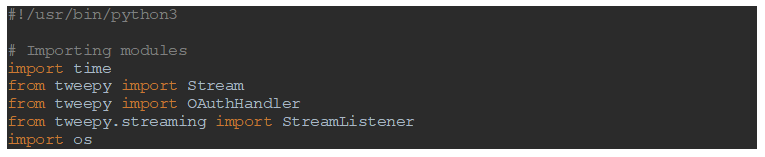
\includegraphics[width=150mm]{code1.png}
	\caption{A simple caption \label{overflow}}
\end{figure}

Apart from the three tweepy class imports that we use to construct the stream listener, the time library will be used to create a time-out feature for the script, and the os library will be used to set your working directory.

\subsection{Setting the Variables:}

\begin{figure}[ht!]
	\centering
	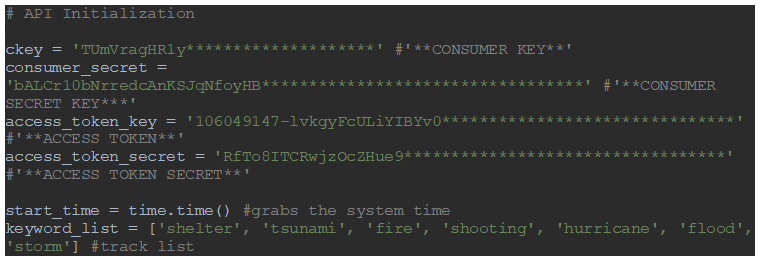
\includegraphics[width=150mm]{code2.png}
	\caption{A simple caption \label{overflow}}
\end{figure}

We have to set the above variables, which will be used in the stream listener by being fed into the tweepy objects.

\subsection{Using and Modifying the Tweepy Classes:}

\begin{figure}[ht!]
	\centering
	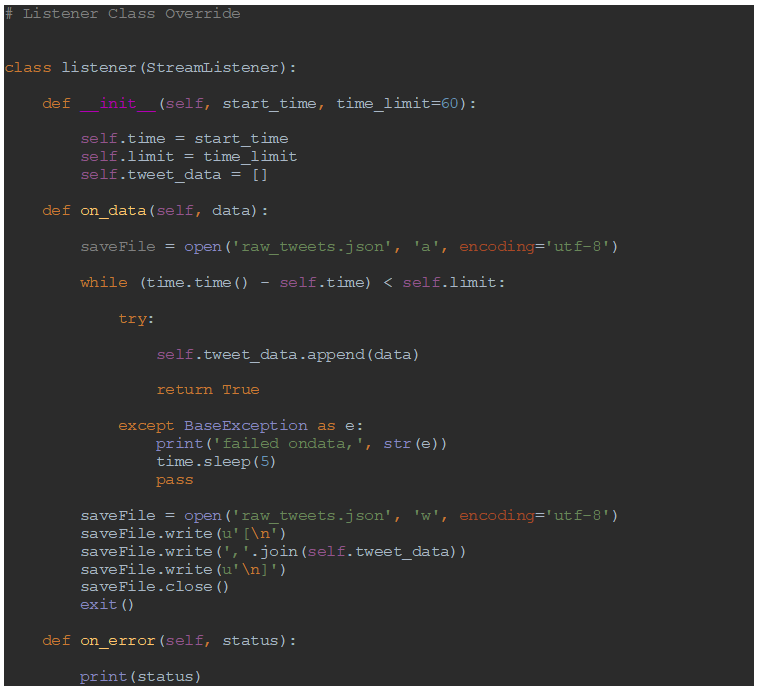
\includegraphics[width=150mm]{code3.png}
	\caption{A simple caption \label{overflow}}
\end{figure}

The code shown below does the following:

\begin{description}
	
\item[$\bullet$]Creates an OAuthHandler instance to handle OAuth credentials

\item[$\bullet$]Creates a listener instance with a start time and time limit parameters passed to it

\item[$\bullet$]Creates an StreamListener instance with the OAuthHandler instance and the listener instance
\end{description}

Before these instances are created, we have to "modify" the StreamListener class by creating a child class to output the data into a .csv file.

We will output the data into MongoDB by reading this csv file.

To elaborate more on the writing of the data to a file after the StreamListener instance receives data:

\begin{figure}[ht!]
	\centering
	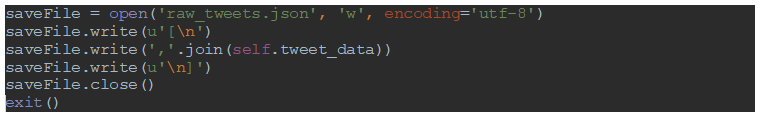
\includegraphics[width=150mm]{code5.png}
	\caption{A simple caption \label{overflow}}
\end{figure}

This block of code opens an output file, writes the opening square bracket, writes the JSON data as text separated by commas, then inserts a closing square bracket, and closes the document. This is the standard JSON format with each Twitter object acting as an element in a JavaScript array. If you bring this into Python built-in parser and the json library can properly handle it.

This section can be modified to or modify the JSON file. For example, we can place other properties/fields like a UNIX time stamp or a random variable into the JSON. We can also modify the output file or eliminate the need for a .csv file and insert the tweet directly into a MongoDB database. As it is written, this will produce a file that can be parsed by Python's json class.

After the child class is created we can create the instances and start the stream listener.

\subsection{Calling the Stream Listener:}

\begin{figure}[ht!]
	\centering
	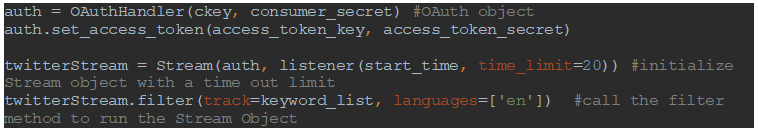
\includegraphics[width=150mm]{code6.png}
	\caption{A simple caption \label{overflow}}
\end{figure}

Here the OAuthHandler uses your API keys [consumer key and consumer secret key] to create the auth object. The access token, which is unique to an individual user [not an application], is set in the following line. This will take all four of your credentials from the Twitter Dev site. The modified StreamListener class simply called listener is used to create a listener instance. This contains the information about what to do with the data once it comes back from the Twitter API call. Both the listener and auth instances are used to create the Stream instance which combines the authentication credentials with the instructions on what to do with the retrieved data. The Stream class also contains a method for filtering the Twitter Stream. The parameters are passed to the Stream API call.

\section{MongoDB}

Storing JSON tweets as a .csv file works well, but they don’t always make good flat .csv files as not every tweet has the same structure nor do every tweet contain the same fields. Some data is well nested into the JSON objects. It is possible to write a parser that has a field for each possible subfield, but this can take a lot of time as involves a lot of considerations and will also create a large .csv file or SQL database.

NoSQL databases like MongoDB greatly simply tweet storage, search and recall which eliminates the need to use an extensive tweet parser.

\subsection{What is MongoDB?}

It is a document-based database that stores data using documents rather than using tuples in tables like traditional relational databases. These documents are similar in structure to JSON objects using key-value pairs and are called BSON (Binary JSON). JSON and BSON have similar properties as JS objects and Python dictionaries.

\subsection{Why store in MongoDB?}

Storing tweets in MongoDB makes sense as BSON and JSON are so similar and that makes putting the entire content of a tweet’s JSON string into an insert statement and executing that statement to store the data. This also makes recalling and searching for tweets simple although it does require a change in thought process of rather executing traditional SQL commands to treating data as OOP structures.

\section{Storing Tweets in MongoDB:}

\begin{figure}[ht!]
	\centering
	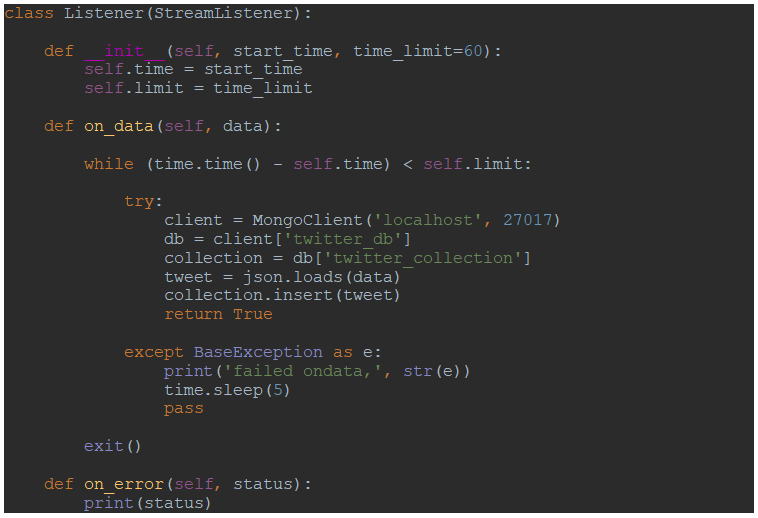
\includegraphics[width=150mm]{code7.png}
	\caption{A simple caption \label{overflow}}
\end{figure}

Once MongoDB is installed and configured storing tweets is simple using the Python stream listener. Modifying the code shown above we have to import pymongo and json libraries. The json library is the default python library and will be available to import, pymongo needs to be set up using the following command:

\$ pip install pymongo

The main changes in the code that I had to do was in the listener child class as shown below.

$MongoClient creates the MongoClient instance which interfaces with the database. The client[‘twitter_db’] call designates the database that is going to be used, and the db[‘twitter_collection’] call selects the collection where the documents will be stored. The json.loads() call converts the string returned from the Twitter API into a json object in Python. Finally, the collection.insert() call inserts the json object into the MongoDB database. From this rather simple change to the Python stream listener all the tweets can be saved into a MongoDB database.
$
\section{Recalling Tweets from MongoDB:}

The function to retrieve any document from a MongoDB database is collection.find(). Here, I can specify what I want or leave it black to get all the documents returned, in my case it will be all the tweets.

Calling using the .find() method, Python returns a MongoDB cursor, which can be iterated through by putting it in a for loop. The for loop will run the loop for each object in the iterator. 

\section{Hadoop:}
%% This is an example first chapter.  You should put chapter/appendix that you
%% write into a separate file, and add a line \include{yourfilename} to
%% main.tex, where `yourfilename.tex' is the name of the chapter/appendix file.
%% You can process specific files by typing their names in at the 
%% \files=
%% prompt when you run the file main.tex through LaTeX.
\chapter{Design and Implementation}

This chapter of the study deals with the design and the implementation of the system being proposed to store disaster-related information. Here, we will look into the specific technologies used to construct the system. This system is intentionally designed to be modular so that specific technologies used can interchanged to provide improvements to the system while also making it possible to adapt the system to different types of use cases.

\begin{figure}[ht!]
	\centering
	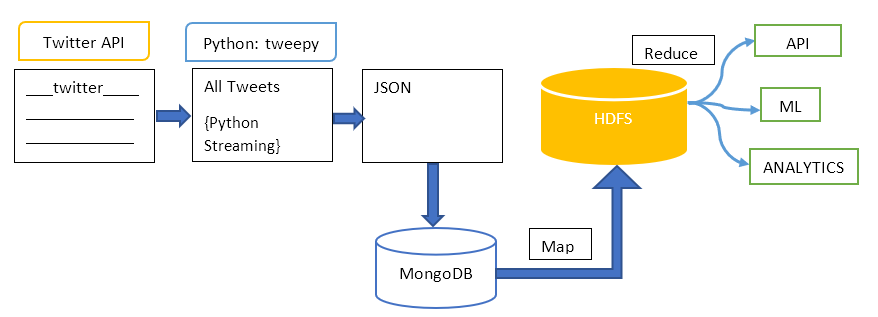
\includegraphics[width=150mm]{DesignDiagram.png}
	\caption{Disaster Management Information System design. \label{overflow}}
\end{figure}

The flow of the Disaster Management Information System design is shown in Figure 3-1. Here the Twitter Streaming API provided by Twitter is incorporated in to the system by using tweepy, a python library, to extract the disaster related data. The Streaming API provides a JSON output which is stored into MongoDB. The output of the MongoDB is parsed using a cognitive filtering system to filter out the irrelevant data and then sent to Hadoop mapper to store all the relevant information in the HDFS data store. Hadoop reduce is used to structure the relevant information and provide it to the end user.

\section{Twitter}

\subsection{Twitter API}\label{ch1:opts}

Twitter as a platform has a lot of users and it generates a lot of data that can be used for analysis. Data can include user tweets, user profiles, user followers, user status, what's trending, etc. This data can be extracted using Twitter Application Programming Interface(API). There are three methods to get this data: the REST API, the search API, and the Streaming API. The Search API is retrospective and allows to search old tweets [with severe limitations], the REST API allows you to collect user profiles, and followers, and the Streaming API collects tweets in real time as they happen. As this study concerns with the real-time analysis of the data, it is important to highlight the fact that the Streaming API is most suited for those needs.

Using the Twitter API requires a few steps:

\begin{enumerate}
  \item Authenticate with OAuth
  \item Make API call
  \item Receive JSON file back
  \item Interpret JSON file
\end{enumerate}

\subsection{Authenticate with OAuth}

OAuth is an open standard for access delegation, commonly used as a way for Internet users to grant websites or applications access to their information on other websites but without giving them the passwords \cite{gordonunderstanding}. Authentication with OAuth on Twitter requires you to get keys from the Twitter developers site using a Twitter developer account. There are four keys (Consumer Key, Consumer Secret Key, Access Token, and Secret Token) that are required to access the API and need to be used during a handshake, once authenticated the program can make API calls.

% This is an example of how you would use tgrind to include an example
% of source code; it is commented out in this template since the code
% example file does not exist.  To use it, you need to remove the '%' on the
% beginning of the line, and insert your own information in the call.
%
%\tagrind[htbp]{code/pmn.s.tex}{Post Multiply Normalization}{opt:pmn}

\subsection{Make API call:}

When making an API call to twitter it has parameters incorporated into the URL, the wrapper looks like this:

\hfill

\url{https://stream.twitter.com/1.1/statuses/filter.json?track=twitter}

\hfill

This call is being done through the streaming API, where it is asking to connect to Twitter and once connection is established it will track the keyword 'twitter'. To track specific information,  keywords can be listed and if done carefully it can filter a lot data at an early stage that is irrelevant in this research. For example, keywords such as 'hurricane', 'flood', 'epidemic', etc., can be listed to stream tweets containing these words.

Using  python library called tweepy the working of an API call is abstracted from the user, nevertheless understanding the working of making a Twitter API call is necessary to extract the relevant data.

% This is an example of how you would use tgrind to include an example
% of source code; it is commented out in this template since the code
% example file does not exist.  To use it, you need to remove the '%' on the
% beginning of the line, and insert your own information in the call.
%
%\tgrind[htbp]{code/be.s.tex}{Block Exponent}{opt:be}

\subsection{Receive JSON file back:}

JavaScript Object Notation (JSON) is an open standard file format that has data formatted as attribute-value pairs. The format is language independent and is commonly used for asynchronous browser-server communication for a data request.

JSON files is also the data structure that Twitter returns when an API call is made. The amount of data returned depends on how the keywords are defined, but is usually rather comprehensive and needs to be parsed.

\subsection{Interpret JSON file:}

JSON file can be stored as raw file or can be stored using a SQL/NoSQL database. Since the data received is unstructured the most logical way to store the data is using a NoSQL database. In this study MongoDB is used to store the tweets we receive and parse through. Next, queries are run based on the keywords that are needed to select information.

\section{Python:}

While there are many different programming languages that can be used to interface with the API, the flexibility and huge community support behind python as well as its relevance in data science makes python the ideal choice in this research. Python has many libraries that has different use cases, here tweepy is used to stream the disaster-related data from twitter.

\section{Tweepy:}

Python is a versatile language with adaptability to various use cases. These are done by extending the language by using libraries which are community created. One of these libraries is tweepy. Tweepy is open-sourced, hosted on GitHub and enables Python to communicate with Twitter platform and use its API \cite{tweepypython}. This makes it easier to access the platform to collect and monitor tweets for analysis.

\subsection{Using tweepy:}

Command to install the tweepy library:

\hfill

\begin{lstlisting}
\$ pip install tweepy
\end{lstlisting}

Tweepy supports OAuth authentication. Authentication is handled by the \\ tweepy.AuthHandler class \cite{tweepyauth}.
A consumer token and a secret key is needed to connect with the Twitter stream API, this uses the keys that were generated after a Twitter developer account was created.

These keys are a pair of private and public (secret and non-secret) keys and used to maintain security. The consumer key pair authorizes the program to use the Twitter API, and the access token essentially signs the application into specific Twitter user account. This framework makes more sense in the context of third party Twitter developers like TweetDeck where the application is making API calls but it needs access to each user's personal data to write tweets, access their time-lines, etc. \cite{collectingtwitter}.

The tweepy library can be imported as shown:

\begin{description}
\item[$\bullet$]from tweepy import Stream

\item[$\bullet$]from tweepy import OAuthHandler

\item[$\bullet$]from tweepy.streaming import StreamListener
\end{description}

The above tweepy class imports will be used to construct the stream listener.


\section{Diving into the code:}

This section helps to describe how the information is stored as a flat file and the advantages of storing the information into a NoSQL data store like MongoDB. Here, the tweepy library is shown using the Streaming API to store information.

\subsection{Importing the modules:}

\begin{figure}[ht!]
	\centering
	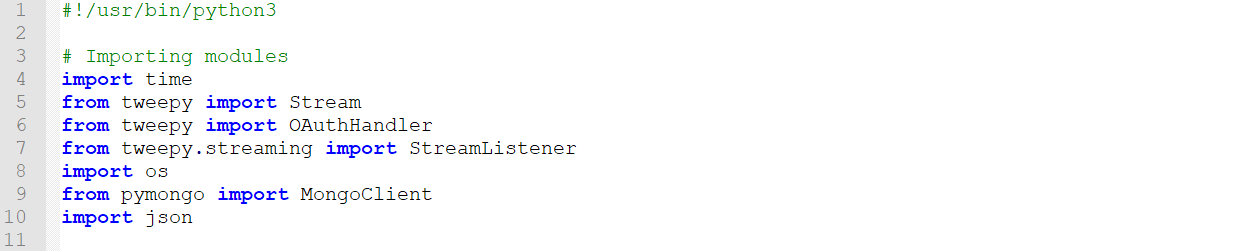
\includegraphics[width=150mm]{code11.png}
	\caption{Importing libraries. \label{overflow}}
\end{figure}

As shown in Figure 3-2, apart from the three tweepy class imports used to construct the stream listener, the time library is used to create a time-out feature for the script, and the os library is used to set the working directory.

\subsection{Setting the Variables:}

\begin{figure}[ht!]
	\centering
	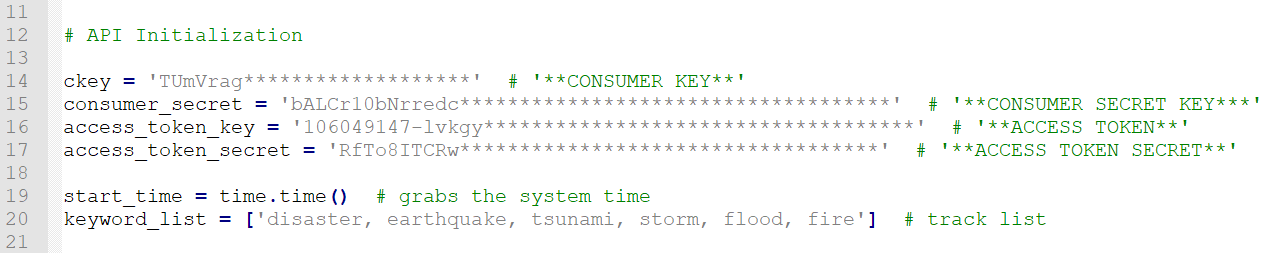
\includegraphics[width=150mm]{code21.png}
	\caption{Setting tokens. \label{overflow}}
\end{figure}

As shown in Figure 3-3, the variables have to be set, which is then used in the stream listener by being fed into the tweepy objects. Here, we set the different token keys generated by signing up for the Twitter API. These keys help to provide access without twitter divulging its authentication tokens.

\subsection{Using and Modifying the Tweepy Classes:}

The code shown in Figure 3-4 does the following:

\begin{figure}[ht!]
	\centering
	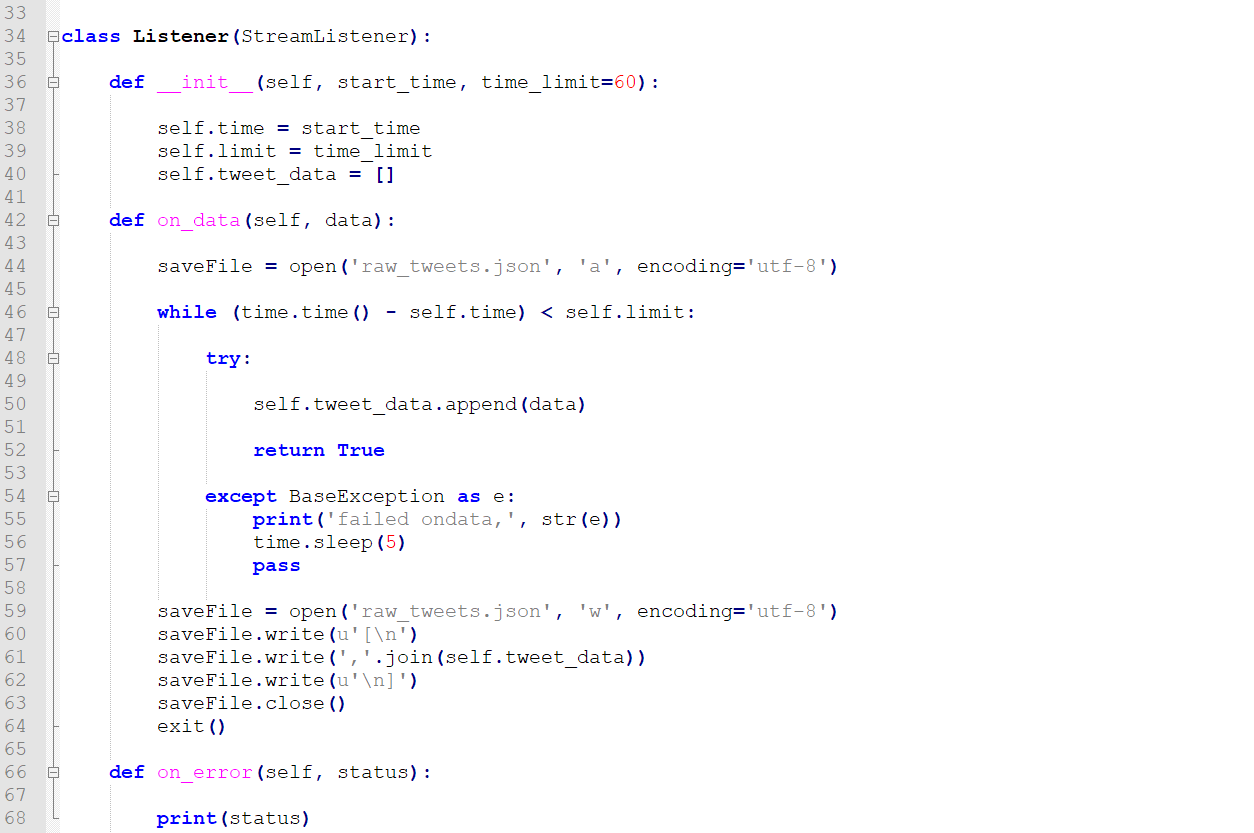
\includegraphics[width=200mm]{code31.png}
	\caption{Stream listener. \label{overflow}}
\end{figure}

\begin{description}
	
\item[$\bullet$]Creates an OAuthHandler instance to handle OAuth credentials.

\item[$\bullet$]Creates a listener instance with a start time and time limit parameters passed to it.

\item[$\bullet$]Creates an StreamListener instance with the OAuthHandler instance and the listener instance.
\end{description}

However, before these instances are created, the StreamListener class has to be modified by creating a child class to output the data into a .csv file. This data is outputted into MongoDB by reading this .csv file. The advantage we gain here is that the data can be queries using the NoSQL data store's querying methods to search for information. This makes it easier to continuously store data on a streaming basis without interrupting the data flow. Also, using a NoSQL data store we can easily without any downtime or interruption to the streaming process.

To elaborate more on the writing of the data to a file after the StreamListener instance receives data:

\begin{figure}[ht!]
	\centering
	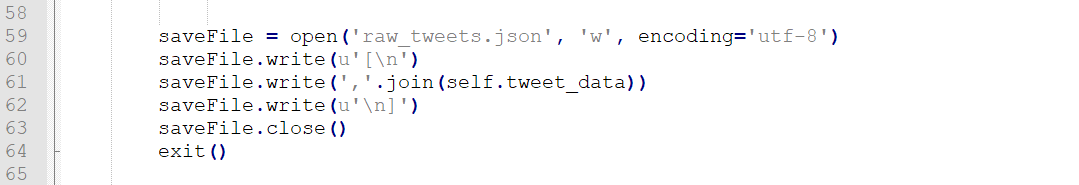
\includegraphics[width=200mm]{code51.png}
	\caption{Storing data. \label{overflow}}
\end{figure}

As shown in Figure 3-5, the block of code opens an output file, writes the opening square bracket, writes the JSON data as text separated by commas, then inserts a closing square bracket, and closes the document. This is the standard JSON format with each Twitter object acting as an element in a JavaScript array. If this is brought into the Python built-in parser, the JSON library can properly handle it.

This section can be modified to or modify the JSON file. For example, other properties/fields like a UNIX time stamp or a random variable can be placed into the JSON format. Additionally, the output file can also be modified to eliminate the need for a .csv file and insert the tweet directly into a MongoDB database. As it is written, this will produce a file that can be parsed by Python's JSON class.

After the child class is created , the instances can be created and then the stream listener can be started to store the information.

\subsection{Calling the Stream Listener:}

\begin{figure}[ht!]
	\centering
	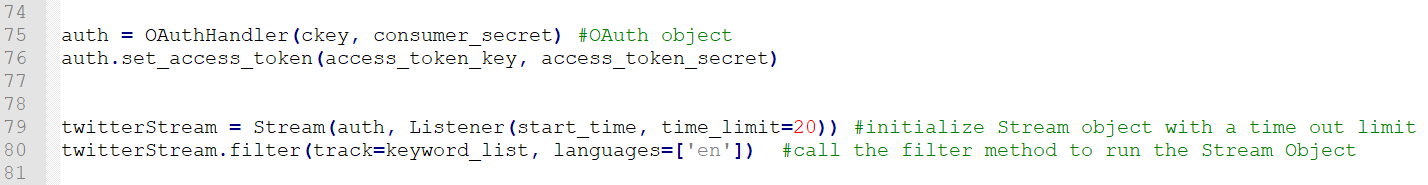
\includegraphics[width=150mm]{code61.png}
	\caption{Calling and filtering tweets in real time. \label{overflow}}
\end{figure}

As shown in Figure 3-6, the OAuthHandler uses the generated API keys [consumer key and consumer secret key] to create the auth object. The access token, which is unique to an individual user [not an application], is set in the following line. This will take all four of the credentials from the Twitter Dev site. The modified StreamListener class, simply called listener, is used to create a listener instance. This contains the information about what to do with the data once it comes back from the Twitter API call. Both the listener and auth instances are used to create the Stream instance which combines the authentication credentials with the instructions on what to do with the retrieved data. The Stream class also contains a method for filtering the Twitter Stream. The parameters are passed to the Stream API call.

\subsection{Twitter Streaming Output:}

Figure 3-7 depicts the output of the Twitter Streaming API, here the keywords used are earthquake, disaster, flood. The output is store to a flat .csv file. In the figure the green highlighted tweets specify the relevant output while the red highlighted tweets show the irrelevant information to this system. This can be parsed by passing the information through a cognitive filtering system.

\begin{figure}[ht!]
	\centering
	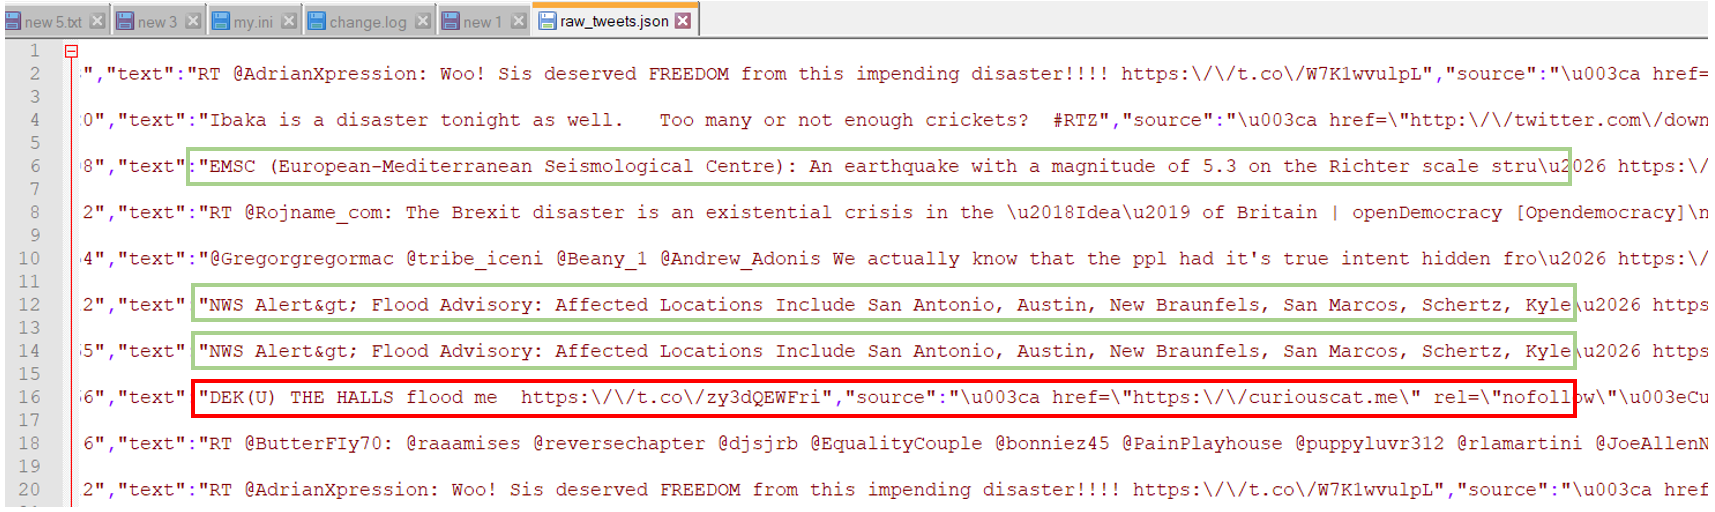
\includegraphics[width=153mm]{tweetoutput.png}
	\caption{Tweet stream output. \label{overflow}}
\end{figure}

\section{MongoDB}

Storing JSON tweets as a .csv file works well, but they don't always make good flat .csv files as not every tweet has the same structure nor do every tweet contain the same fields. Some data is well nested into the JSON objects. It is possible to write a parser that has a field for each possible subfield, but this can take a lot of time as involves a lot of considerations and will also create a large .csv file or SQL database.

NoSQL databases like MongoDB works very well as a simple tweet storage, search and recall, which eliminates the need to use an extensive tweet parser.

\subsection{What is MongoDB?}

It is a document-based database that stores data using documents rather than using tuples in tables like traditional relational databases. These documents are similar in structure to JSON objects using key-value pairs and are called BSON (Binary JSON). JSON and BSON have similar properties as JS objects and Python dictionaries.

\subsection{Why store in MongoDB?}

Storing tweets in MongoDB makes sense as BSON and JSON are so similar and that makes putting the entire content of a tweet's JSON string into an insert statement and executing that statement to store the data. This also makes recalling and searching for tweets simple although it does require a change in thought process of rather executing traditional SQL commands to treating data as OOP structures.

\section{Storing Tweets in MongoDB}

\begin{figure}[ht!]
	\centering
	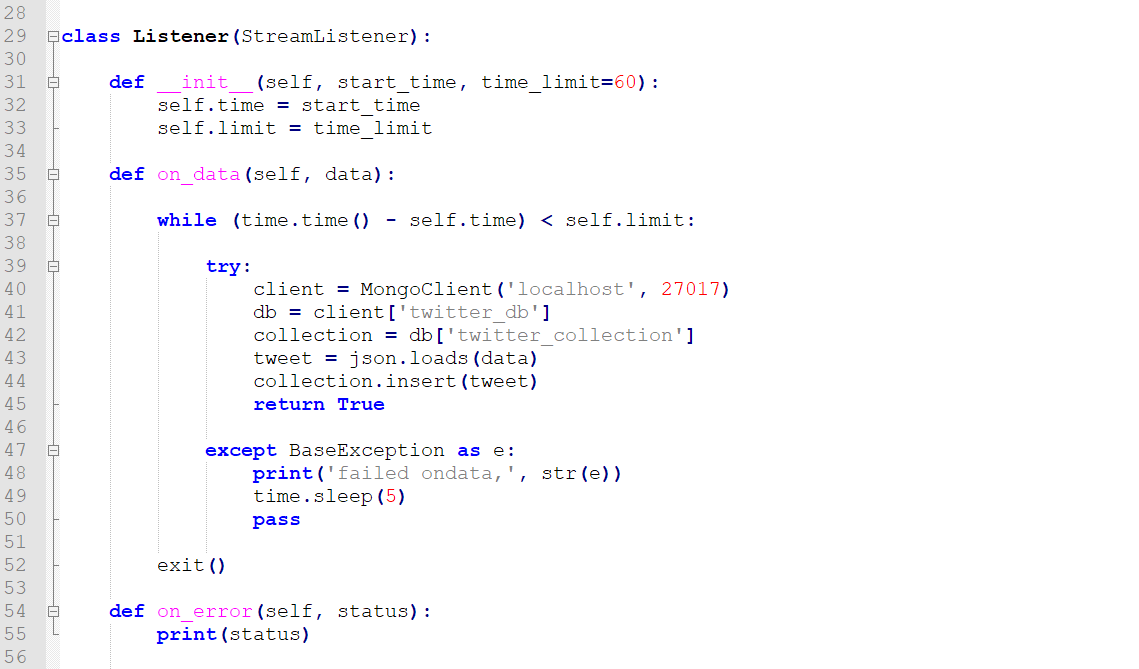
\includegraphics[width=200mm]{code71.png}
	\caption{Storing tweets in MongoDB. \label{overflow}}
\end{figure}

Once MongoDB is installed and configured storing tweets is simple using the Python stream listener. Modifying the code shown above the pymongo and JSON libraries can be imported. The JSON library is the default python library and will be available to import, pymongo needs to be set up using the following command:

\begin{lstlisting}
\$ pip install pymongo
\end{lstlisting}

The main changes in the code that was done is in the listener child class as shown in Figure 3-7.

as  shown in Figure 3-8, MongoClient creates the MongoClient instance which interfaces with the database. The client['twitter\_db'] call designates the database that is going to be used, and the db['twitter\_collection'] call selects the collection where the documents will be stored. The json.loads() call converts the string returned from the Twitter API into a JSON object in Python. Finally, the collection.insert() call inserts the JSON object into the MongoDB database. From this rather simple change to the Python stream listener all the tweets can be saved into a MongoDB database.

\section{Recalling Tweets from MongoDB}

The function to retrieve any document from a MongoDB database is collection.find(). Here, I can specify what I want or leave it black to get all the documents returned, in my case it will be all the tweets.

Calling using the .find() method, Python returns a MongoDB cursor, which can be iterated through by putting it in a for loop. The for loop will run the loop for each object in the iterator. 

\section{Context based filtering}

Context-based filtering, also referred to as cognitive filtering, recommends elements based on a comparison between the content of the elements and the requirement of the output. Content of each element is represented as a set of descriptors or terms, typically a set of words that occur in a document or in this case in the data stored in MongoDB.

\begin{figure}[ht!]
	\centering
	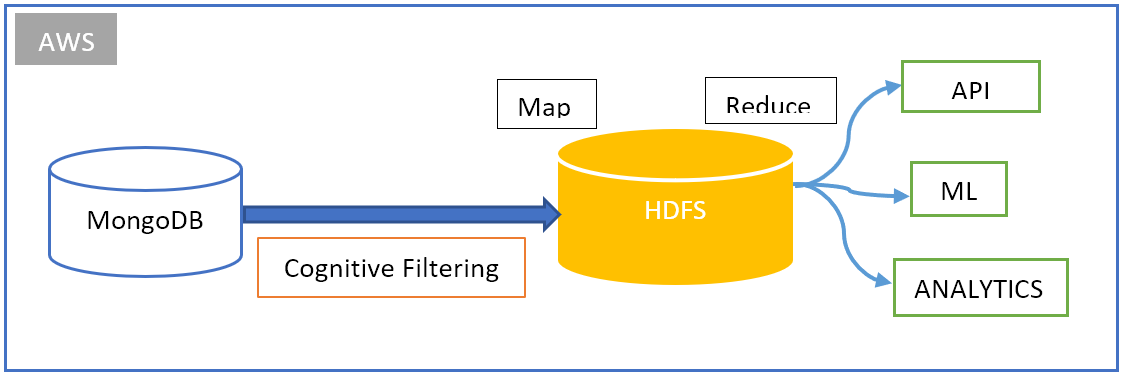
\includegraphics[width=150mm]{ContextFiltering.png}
	\caption{Cognitive filtering model. \label{overflow}}
\end{figure}

As shown in Figure 3-9, the cognitive filtering system will filter relevant information from the Streaming API output as shown in Figure 3-7. The cognitive filtering model can represent each disaster element as a set of terms that can be based on the context of the output to filter out the information.

\begin{figure}[ht!]
	\centering
	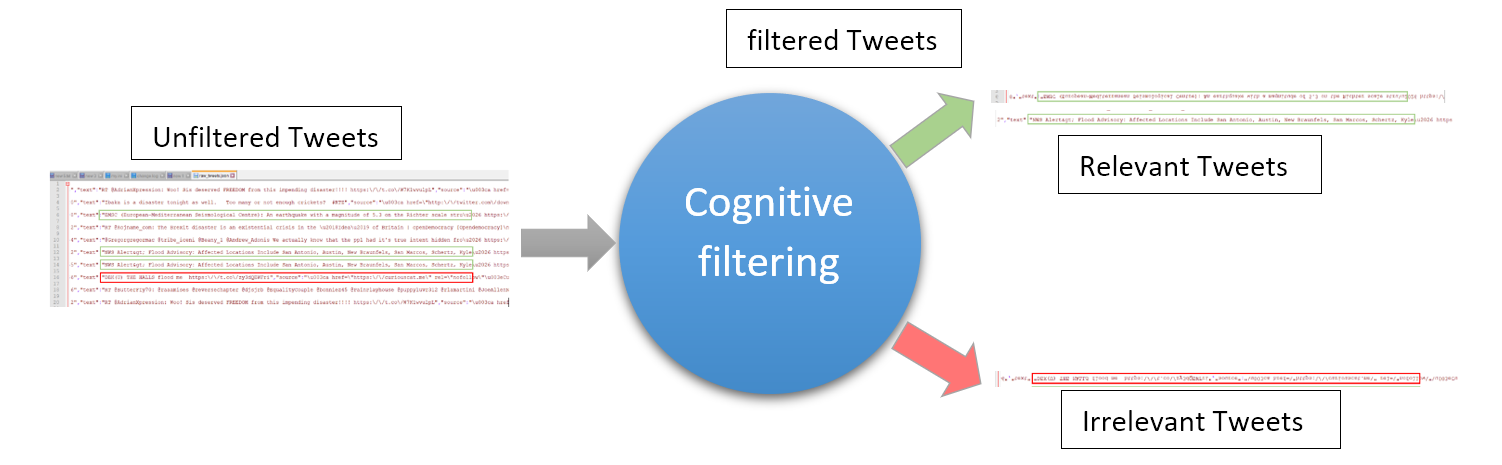
\includegraphics[width=150mm]{ContextFilteringWorking.png}
	\caption{Cognitive filtering model. \label{overflow}}
\end{figure}

As shown in Figure 3-10, the context filtering model works to filter the tweets base on relevance of the information being fed to it. The model is trained to understand the context of the data and provide output based on those requirements. With respect to filtering the disaster related data, the model takes the unfiltered data and filters the data into relevant and irrelevant information. The relevant information is sent to the Hadoop data store for further processing, the irrelevant information is discarded, saving space.

Although, it is out of scope of this research to implement a context-based filtering system, it is absolutely necessary to mention a need of a cognitive based system to filter the data before processing it, as the goal of the DMIS design is to provide a solution for fast delivery during response phase of a disaster.

\section{Hadoop}

Hadoop is a programming framework used to support the processing of large data sets in a distributed computing environment \cite{shvachko2010hadoop}. Hadoop ecosystem consists of Hadoop Kernel, Mapreduce, HDFS and number of various components like Apache Hive, Base and Zookeeper.

This study uses MapReduce framework to process the data to output the information. The framework allows processing of large dataset by using divide and conquer strategy, and run it in parallel.

The input of the Hadoop data store is the output of the context filtering model. The relevant tweets are stored in the data store. The system processes the tweets using Hadoop Map and Reduce to provide location-based information.

\section{Amazon Web Services}

Amazon Web Services (AWS), a cloud computing service, provides a platform that is ideally suited for building fault-tolerant software systems \cite{barr2011building}. As the DMIS platform aims to be operational even during a disaster, hosting it on cloud platform like AWS is a logical choice.

Amazon Elastic Compute Cloud (Amazon EC2) is a web service within AWS that provides computing resources that can be used to build and host systems. Using multiple EC2 instances, a highly reliable and fault-tolerant DMIS can be built. Also AWS provides the flexibility to scale using tools and ancillary services such as Auto Scaling and Elastic Load Balancing.

On the surface, Amazon EC2 instances behave like traditional hardware servers as they provide a virtual shell to host familiar operating systems like Linux, Windows, or Debian. Thus, providing flexibility to accommodate any type of platform to run on these systems. Additionally, a system can start small and grow when needed by adding heterogeneous nodes.

Using AWS, DMIS is poised to realize the full potential of the platform and use its services in the fullest possible way. Furthermore, gradual expansion of the system can be modular and new features can be incorporated in to the system over new nodes.

\section{Summary}

In this chapter the design of the system was described while also detailing the choices made to use certain technologies to implement the system in practice. The twitter data streaming API called the Twitter Streaming API is used and integrated in to the tweepy python library to abstract the API call for easier implementation.

The Streaming data is stored in a .csv file which is then read into MongoDB to store the information. During the streaming API call the Twitter Streaming API provides the option to extract data based on keywords. This is specified during the DMIS API call and is the first step to filter the data collected from the Twitter data store.

As the data collected is still unfiltered as it contains relevant information mixed with irrelevant information, the system has to filter this before processing it further. This is done before the data is passed to Hadoop for further processing. The unfiltered data is passed through a cognitive filtering system to sort the data based on the context of the information. The cognitive filtering model works as shown in Figure 3-10.

Once the data is filtered the relevant information is passed to the Hadoop system for processing, the Hadoop map and reduce functions are used to parse the information and structure the data that can be queried using an API call to serve different use cases. Additionally, the raw information can be provided that can be used for further analysis or parsing as needed.

All the components of the system are hosted on Amazon Web Services cloud computing platform for making it resilient to disaster related failures. In the context of this study, the system described here provides with an approach to a system that can parse disaster related data and store it continuously.
\appendix
\chapter{Tables}

\begin{table}
\caption{Armadillos}
\label{arm:table}
\begin{center}
\begin{tabular}{||l|l||}\hline
Armadillos & are \\\hline
our	   & friends \\\hline
\end{tabular}
\end{center}
\end{table}

\clearpage
\newpage

\chapter{Figures}

\vspace*{-3in}

\begin{figure}
\vspace{2.4in}
\caption{Armadillo slaying lawyer.}
\label{arm:fig1}
\end{figure}
\clearpage
\newpage

\begin{figure}
\vspace{2.4in}
\caption{Armadillo eradicating national debt.}
\label{arm:fig2}
\end{figure}
\clearpage
\newpage

%% This defines the bibliography file (main.bib) and the bibliography style.
%% If you want to create a bibliography file by hand, change the contents of
%% this file to a `thebibliography' environment.  For more information 
%% see section 4.3 of the LaTeX manual.
\begin{singlespace}
\bibliography{main}
\bibliographystyle{plain}
https://www.pythoncentral.io/introduction-to-tweepy-twitter-for-python/

$https://github.com/tweepy/tweepy/blob/v3.6.0/docs/auth_tutorial.rst
$
https://lifehacker.com/5918086/understanding-oauth-what-happens-when-you-log-into-a-site-with-google-twitter-or-facebook

\end{singlespace}

\end{document}

